%!TeX root = main.tex
% TODO; wie darf ich einen Meromorphen verändern, (das P verändern) ohne das
% sich effektiv was ändert?
% TODO: \cM = \cM_K ... replace
% TODO: Dimension eines Meromorphen Zusammenhang
\chapter{Meromorphe Zusammenhänge}
Sei $\cM$ ein $\cD$-Modul ungleich Null von endlichem Typ. Falls die
links-Multiplikation mit $x$ bijektiv ist, so nennen wir $\cM$ einen
Meromorphen Zusammenhang. \cite[Chap 4]{sabbah_cimpa90}

\section{Systeme von ODEs und Meromorphe Zusammenhänge}
%TODO: \tilde cO --> \tilde \cO
\cite[Chap 5.1.1]{hotta2007d} %abgeschrieben
Für eine Matrix $A(x)=(a_{ij}(x))_{ij}\in M(n\times n,K)$ betrachten wir das
System von gewöhnlichen Differentialgleichungen (kurz ODEs)
\begin{equation}
\label{eq:KlassischesODE}
%TODO: partial oder d
\frac{d}{dx}u(x)=A(x)u(x)
\end{equation}
wobei $u(x)=\,^t(u_1(x),\dots,u_n(x))$ ein Spaltenvektor von unbekannten
Funktionen. Wir werden (\ref{eq:KlassischesODE}) immer in einer Umgebung um
$x=0\in\C$ betrachten. Als Lösungen von (\ref{eq:KlassischesODE}) betrachten
wir Keime von holomorphen (aber möglicherweise mehrdeutigen)
 %but possibly multivalued auf
Funktionen an $x=0$ (geschrieben als $\tilde\cO$).
%auf der punktierten Scheibe
%$B_\epsilon^*=\{x\in\C|0<|x|<\epsilon\}$, wobei $\epsilon>0$ klein genug sei.
 Wir sagen $v(x)=\,^t(v_1(x),\dots,v_n(x))$ ist
eine Lösung von (\ref{eq:KlassischesODE}), falls $ v_i\in\tilde \cO$ für alle
$i\in\{1,\dots,n\}$ und $v$ die Gleichung (\ref{eq:KlassischesODE}),
auf einer Umgebung um die $0$, erfüllt.

\begin{comment}
TODO: zeige, das der lösungsraum die eigenschaften von $\cD$-Moduln erfüllt\\
siehe alternativer Zugang
\end{comment}

\subsubsection{Alternativer Zugang}
\begin{comment}
Sei $P$ ein linearer Differentialoperator mit Koeffizienten in $a_i(x)\in\Ckx$
geschrieben als $P=\sum^{d}_{i=0}{a_{i}(x)\partial_x^i}$.
Man sagt eine Funktion $u\in\cF$ ist Lösung von $P$, falls $u$ die Gleichung
$Pu=0$ erfüllt.
Man sagt $0$ ist ein singulärer Punkt falls $a_d(0)=0$.
Falls $0$ kein singulärer Punkt ist, hat $P$ genau $d$ über $\C$ Unabhängige
Lösungen in $\Ckx$. %TODO: oder \tilde\cO
\end{comment}

\cite[3.1.1]{sabbah_cimpa90} Sei $\cF$ ein Funktionenraum, auf dem die
Differentialoperatoren $\cD$ wirken. Ein Element $u\in \cF$ ist Lösung von
$P\in\cD$ falls $P\cdot u=0$ gilt.

Falls $u$ ein Lösung von $P$ ist, so ist $u$ auch Lösung von $Q\cdot P$ mit
$Q\in \cD$. Also hängt die Lösung nur vom Links Ideal $\cD\cdot
P\vartriangleleft\cD$ ab.

\subsection{Meromorphe Zusammenhänge}
Nun wollen wir dieses Klassische Gebilde nun in die moderne Sprache der
Meromorphen Zusammenhänge übersetzen.
%\section{Meromorpher Zusammenhang (Definition)}
%Quelle ist \cite{sabbah_cimpa90}
\begin{defn}[Meromorpher Zusammenhang] \label{def:merom-zush}
Ein \emph{Meromorpher Zusammenhang} (bei $x=0$) ist ein Tuppel
$(\cM_K,\partial)$ und besteht aus folgenden Daten:
\begin{itemize}
\item $\cM_K$, ein endlich dimensionaler $K$-Vektor Raum
\item einer $\C$-linearen Abbildung $\partial:\cM_K\rightarrow \cM_K$,
genannt \emph{Derivation} oder \emph{Zusammenhang}, welche für alle $f\in K$
und $u\in \cM_K$ die \emph{Leibnitzregel}
\begin{equation}\label{eq:Leibnitzregel}
\partial(fu)=f'u+f\partial u %TODO: hier klammern um das letzte u ?
\end{equation}
erfüllen soll.
\end{itemize}
\end{defn}
\begin{bem}[Formaler Meromorpher Zusammenhang]
Analog definiert man einen \emph{formalen Meromorphen Zusammenhang}
$(\cM_{\hat K},\partial)$ bestehend, analog wie in Definition
\ref{def:merom-zush}, aus folgenden Daten:
\begin{itemize}
\item $\cM_{\hat K}$, ein endlich dimensionaler $\hat K$-Vektor Raum
\item einer $\C$-linearen Derivation $\partial:\cM_{\hat K}\rightarrow
\cM_{\hat K}$, welche die \emph{Leibnitzregel} (\ref{eq:Leibnitzregel})
erfüllen soll.
\end{itemize}
\end{bem}

\begin{defn}
Seien $(\cM_K,\partial_\cM)$ und $(\cN_K,\partial_\cN)$ zwei Meromorphe
Zusammenhänge. Eine $K$-lineare Abbildung $\phi:\cM\rightarrow\cN$ heißt
Morphismus von Meromorphen Zusammenhängen, falls sie
$\phi\circ\partial_\cM=\phi\circ\partial_\cN$ erfüllt. In diesem Fall schreiben
wir auch $\phi:(\cM_K,\partial_\cM)\rightarrow(\cN_K,\partial_\cN)$.
\end{defn}
\begin{comment}
TODO: Wann sind die Isomorph\\
$\cM\cong \cN$ und die Ableitungen kommutieren mit dem Isomorphismus
\end{comment}

\begin{defn}
Wir erhalten damit die Kategorie dier meromorphen Zusammenhänge über $\hat K$
mit 
\begin{align*}
\text{Objekte: } & ()
\end{align*}
\end{defn}

\begin{bem}
\begin{enumerate}
\item Später wird man auf die Angabe von $\partial$ verzichten und einfach
$\cM_K$ als den Meromorphen Zusammenhang bezeichnen, auch wird manchmal auf die
Angabe von $K$ verzichtet.
\item \cite[Rem 5.1.2.]{hotta2007d}
Die Bedingung (\ref{eq:Leibnitzregel}) ist zur schwächeren Bedingung
\[
\partial(fu)=f'u+f\partial u \,,
\]
welche für alle $f\in \tilde\cO$ und für alle $u\in \cM_K$ erfüllt sein muss,
äquivalent.
\end{enumerate}
\end{bem}

\begin{defn}[Zusammenhangsmatrix] \cite[Seite 129]{hotta2007d}
Sei $(\cM_K,\partial)$ ein Meromorpher Zusammenhang so wähle eine $K$-Basis
$\{e_i\}_{i\in\{1,\dots,n\}}$ von $\cM$. Dann ist die
\emph{Zusammenhangsmatrix bzgl. der Basis $\{e_i\}_{i\in\{1,\dots,n\}}$} die
Matrix $A(x)=(a_{ij}(x))\in M(n\times n,K)$ definiert durch
%\[ \partial e_j=-\sum_{i=1}^na_{ij}(x)e_i \,. \]
\[ a_{ij}(x) = -^te_i \partial e_j \,. \]
\end{defn}

Also ist, bezüglich der Basis $\{e_i\}_{i\in\{1,\dots,n\}}$, die Wirkung von
$\partial$ auf $u=:\,^t(u_1,\dots,u_n)$ beschrieben durch
\[
\partial(u) = \partial \Big( \sum_{i=1}^nu_i(x)e_i \Big)
\overbox{=}{??}\sum_{i=1}^n \Big( u_i'(x)-
\sum_{j=1}^na_{ij}u_j(x) \Big)e_i \,.
\]
Einfache Umformungen zeigen, dass die Bedingung $\partial u(x)=0$, für
$u(x)\in \sum_{i=1}^n u_ie_i\in \tilde \cO \otimes_K\cM$, äquivalent zu der
Gleichung
\begin{equation*}
u'(x)=A(x)u(x)
\end{equation*}
für $u(x)=\,^t(u_1(x),\dots,u_n(x))\in\tilde \cO^n$. Damit haben wir gesehen,
dass jeder Meromorphe Zusammanhang $(\cM,\partial)$ ausgestattet mit einer
$K$-Basis $\{e_i\}_{i\in\{1,\dots,n\}}$ von $\cM$ zu einem ODE zugeordnet
werden kann.

Umgekehrt können wir für jede Matrix $A(x)=(a_{ij}(x))$ den
assoziierten Meromorphen Zusammenhang $(\cM_A,\partial_A)$ %TODO: improve notation
angeben, durch
\begin{align*}
\cM_A & :=\bigoplus_{i=1}^n Ke_i \,, & \partial_A e_i &:=
-\sum_{i=1}^na_{ij}(x)e_i \,.
\end{align*}

\section{Eigenschaften / Äquivalenz zu holonomen lokalisierten $\cD$-Moduln}
%Hier nun einige Eigenschaften Meromorpher Zusammenhänge.
\begin{comment}
\cite[4.2]{sabbah_cimpa90}
Let $\cM$ be a left $\cD$-module. First we consider it only as a
$\C\{x\}$-module and let $\cM[x^{-1}]$ be the localized module.
\end{comment}

%TODO: reihenfolge bei sabbah anderst!!!
\begin{lem}[Lemma vom zyklischen Vektor] \label{lem:Zyklischer-Vektor}
\cite[Thm 4.3.3]{sabbah_cimpa90}
\cite[Satz 4.8]{ZulaBarbara}
Sei $\cM_K$ ein Meromorpher Zusammenhang. Es Existiert ein Element
$m\in\cM_K$ und eine ganze Zahl $d$ so dass
$m,\partial_xm,\dots,\partial_x^{d-1}m$ eine $K$-Basis von $\cM_K$ ist.
\end{lem}
\begin{proof}
\cite[Satz 4.8]{ZulaBarbara}
\end{proof}
\begin{comment}
TODO: Wie findet man einen Zyklischen Vektor\\
TODO: wie bekommt man daraus das $P$
\end{comment}

\begin{thm}
\cite[Thm 4.3.2]{sabbah_cimpa90}
Ein Meromorpher Zusammenhang bestimmt ein holonomes lokalisiertes $\cD_K$-Modul
und andersherum.
\end{thm}
\begin{proof}
\cite[Thm 4.3.2]{sabbah_cimpa90}
\end{proof}

\begin{lemdef}
\cite[Satz 4.12]{ZulaBarbara}
\cite[Thm 4.3.2]{sabbah_cimpa90}
Ist $\cM_K$ ein Meromorpher Zusammenhang, dann existiert ein $P\in\cD_K$ so
dass $\cM_K\cong\cD_K/\cD_K\cdot P$. So ein $P$ heißt dann
\emph{Minimalpolynom} von
$\cM_K$.
\end{lemdef}
\begin{proof}
\cite[Satz 4.12]{ZulaBarbara}
\end{proof}
\begin{comment}
\begin{rem}
\cite[Proof of Theorem 5.4.7]{sabbah_cimpa90}
\[
\dim_{\hat K}\cM_{\hat K} =\deg P \mbox{ wenn } \cM_{\hat K}=\cD/\cD\cdot P
\]
\end{rem}
\end{comment}
\begin{thm}\label{thm:basic-splitting}
\cite[Seite 64]{ZulaBarbara} %TODO: hat die sich hier verschrieben???
Ist $P=P_1\cdot P_2$ mit $P_1,P_2\in \cD_K$ so gilt
\[
\cD_K/\cD_K\cdot P \cong \cD_K/\cD_K\cdot P_1 \oplus \cD_K/\cD_K\cdot P_2 \,.
\]
\end{thm}
\begin{proof}
\cite[Seite 57-64]{ZulaBarbara}
\end{proof}
\begin{cor}
Sei $P=P_1\cdot P_2$ mit $P_1,P_2\in \cD_K$ wie in Satz
\ref{thm:basic-splitting} so gilt
\[
\cD_K/\cD_K\cdot (P_1\cdot P_2) \cong \cD_K/\cD_K\cdot (P_2 \cdot P_1)
\]
\end{cor}
\begin{proof}
\begin{align*}
\cD_K/\cD_K\cdot P &= \cD_K/\cD_K\cdot (P_1\cdot P_2)\\
  &\cong \cD_K/\cD_K\cdot P_1 \oplus \cD_K/\cD_K\cdot P_2\\
  &= \cD_K/\cD_K\cdot P_2 \oplus \cD_K/\cD_K\cdot P_1\\
  &\cong \cD_K/\cD_K\cdot (P_2 \cdot P_1)
\end{align*}
\end{proof}

\begin{lem}
Sei $(\cM_K,\partial)$ ein gegebener Meromorpher Zusammenhang, und $\phi$ ein
Basisisomorphismus von $K^r$ nach $\cM_K$, also in der Situation
\begin{center}
\begin{tikzpicture} [scale=3.3, descr/.style={fill=white,inner sep=2.5pt} ]
\matrix (m) [
  matrix of math nodes
  , row sep=3em
  , column sep=3em
  %, text height=3em
  %, text depth=0.25em
]
{
  \cM_K & \cM_K \\
  K^r   & K^r \\
};
\path[->,font=\scriptsize,>=angle 90]
(m-1-1) edge node[above]{$\partial$} (m-1-2)
(m-2-1) edge node[above]{$\phi^{-1}\circ\partial\circ\phi$} (m-2-2)
;
%TODO: make this harpoon arrows
\path[->,font=\scriptsize,>=angle 90]
(m-2-1) edge node[descr]{$\cong$} node[right]{$\phi$} (m-1-1)
(m-2-2) edge node[descr]{$\cong$} node[left]{$\phi$} (m-1-2)
;

\path[>=stealth,|->]
;
\end{tikzpicture}
\end{center}
gilt: $(K^r,\phi^{-1}\circ\partial\circ\phi)$ ist ebenfalls ein Meromorpher Zusammenhang.
\end{lem}
\begin{proof}
TODO, (3. Treffen)
\end{proof}
\begin{comment} %Allgemeiner
\begin{lem}
Sei $(\cM_K,\partial)$ ein gegebener Meromorpher Zusammenhang, und
$\phi:\cM\rightarrow\cN$ ein Isomorphismus so ist
$(\cN,\phi^{-1}\circ\partial\circ\phi)$ ein zu $(\cM_K,\partial)$ isomorpher
Zusammenhang.
\begin{center}
\begin{tikzpicture} [scale=3.3, descr/.style={fill=white,inner sep=2.5pt} ]
\matrix (m) [
  matrix of math nodes
  , row sep=3em
  , column sep=3em
  %, text height=3em
  %, text depth=0.25em
]
{
  \cM_K & \cM_K \\
  \cN   & \cN \\
};
\path[->,font=\scriptsize,>=angle 90]
(m-1-1) edge node[above]{$\partial$} (m-1-2)
(m-2-1) edge node[above]{$\phi^{-1}\circ\partial\circ\phi$} (m-2-2)
;
%TODO: make this harpoon arrows
\path[->,font=\scriptsize,>=angle 90]
(m-2-1) edge node[descr]{$\cong$} node[right]{$\phi$} (m-1-1)
(m-2-2) edge node[descr]{$\cong$} node[left]{$\phi$} (m-1-2)
;

\path[>=stealth,|->]
;
\end{tikzpicture}
\end{center}
\end{lem}
\begin{proof}
TODO, (3. Treffen)
\end{proof}
\end{comment}

\begin{lem} Sei $\cM_K$ %\cong K^r
 ein endlich dimensionaler $K$-Vektor Raum mit $\partial_1$ und $\partial_2$
zwei darauf definierte Derivationen. So gilt, die differenz zweier
Derivationen ist $K$-linear.
\end{lem}
\begin{proof}
Seien $\partial_1$ und $\partial_2$ zwei Derivationen auf $\cM_K$.
Da $\partial_1$ und $\partial_2$ $\C$-linear, ist $\partial_1-\partial_2$
$\C$-linear, also muss nur noch gezeigt werden, dass
$(\partial_1-\partial_2)(fu)=f\cdot(\partial_1-\partial_2)(u)$ $\forall f\in
K$ und $u\in\cM_K$ gilt.\\
%TODO: wieso gilt das?
\begin{align*}
(\partial_1-\partial_2)(fu) &= \partial_1(fu)-\partial_2(fu)\\
&= f'u+f\partial_1u-f'u-f\partial_2u\\
&= \underset{=0}{\underbrace{f'u-f'u}}+f\cdot(\partial_1u-\partial_2u)\\
&= f\cdot(\partial_1-\partial_2)(u)\\
\end{align*}
\end{proof}
\begin{cor}
Für $(K^r,\partial)$ ein Meromorpher Zusammenhang existiert ein $A\in M(r\times
r,K)$, so dass $\partial=\frac{d}{dx}-A$.
\end{cor}
\begin{proof}
Es sei $(K^r,\partial)$ ein Meromorpher Zusammenhang.  So ist
$\frac{d}{dx}-\partial:K^r\rightarrow K^r$ $K$-linear, also lässt sich durch
eine Matrix $A\in M(r\times r,K)$ darstellen
%$\frac{d}{dx}-\partial=A$
, also ist, wie
behauptet, $\partial=\frac{d}{dx}-A$.
\end{proof}

%TODO: beobachtung...

%TODO: differenz ist linear

\begin{prop}[Transformationsformel] \cite[Chap 5.1.1]{hotta2007d}
In der Situation

\begin{center}
\begin{tikzpicture} [scale=3.3, descr/.style={fill=white,inner sep=2.5pt} ]
\matrix (m) [
  matrix of math nodes
  , row sep=3em
  , column sep=3em
  %, text height=3em
  %, text depth=0.25em
]
{
  K^r &   &   & K^r \\
      & M & M & \\
  K^r &   &   & K^r \\
};
\path[->,font=\scriptsize,>=angle 90]
(m-1-1) edge node[descr]{$\cong$} node[above]{$\phi$} (m-2-2)
(m-3-1) edge node[descr]{$\cong$} node[above]{$\psi$} (m-2-2)
(m-1-4) edge node[descr]{$\cong$} node[above]{$\phi$} (m-2-3)
(m-3-4) edge node[descr]{$\cong$} node[above]{$\psi$} (m-2-3)

(m-2-2) edge node[above]{$\partial$} (m-2-3)

(m-1-1) edge node[above]{$\frac{d}{dz}+A$} (m-1-4)
(m-3-1) edge node[above]{$\frac{d}{dz}+B$} (m-3-4)

(m-3-1) edge node[descr]{$\cong$} node[right]{$T$} (m-1-1)
(m-3-4) edge node[descr]{$\cong$} node[left]{$T$} (m-1-4)
;

\path[>=stealth,|->]
;
\end{tikzpicture}
\end{center}
mit $\phi,\psi$ und $T$ $K$-Linear und $\partial,(\frac{d}{dx}+A)$ und
$(\frac{d}{dx}+B)$ $\C$-Linear, gilt:\\
Der Meromorphe Zusammenhang. $\frac{d}{dx}+A$ auf $K^r$ wird durch Basiswechsel
$T\in GL(r,K)$ zu
\[
\frac{d}{dx}+(T^{-1}\cdot T'+T^{-1}AT) = \frac{d}{dx}+B
\]
\end{prop}
\begin{defn}[Differenziell Äquivalent]
Man nennt $A$ und $B$ \emph{differenziell Äquivalent} ($A\sim B$) genau
dann, wenn es ein $T\in
GL(r,K)$ gibt, mit $B=T^{-1}\cdot T'+T^{-1}AT$.
\end{defn}

\begin{comment}
$1=TT^{-1}$ $\rightsquigarrow$ $T'T^{-1}+T(T^{-1})'=0$\\
$1=T^{-1}T$ $\rightsquigarrow$ $(T^{-1})'T+T^{-1}T'=0$
\end{comment}

\begin{prop} \cite[Prop 4.1.1]{SchneidersDmod}
Seien $(\cM,\partial_\cM)$ und $(\cN,\partial_\cN)$ Meromorphe Zusammenhänge.
Durch setzten von
\[
\partial(m\otimes n)=\partial_\cM(m)\otimes n +m\otimes \partial_\cN(n)
\]
als die Wirkung von $\partial$ auf das $K$-Modul $\cM\otimes_K\cN$, wird
$(\cM\otimes_K\cN,\partial)$ zu einem Meromorphen Zusammenhang.
\end{prop}
\begin{proof}
Klar
\end{proof}
\begin{lem} \cite[Ex 5.3.7]{sabbah_cimpa90}
%TODO: move after slope definition!!!
Falls $\cN$ regulär und nicht Null, dann ist die Menge der Slopes von
$\cM\otimes\cN$ genau die Menge der Slopes von $\cM$.
\end{lem}
\begin{proof}
TODO
\end{proof}

\section{Newton Polygon}
% ist dies eine Invariante??
% gestohlen aus der ZulaBarbara Seite 46
\begin{comment}
Quelle: sabbah?\\
sabbah mach alles formal, barbara mach alles konvergent
\end{comment}
Jedes $P\in \cD_{\hat K}$, also insbesondere auch jedes $P\in\cD_K$, lässt sich
eindeutig als
\[
P=\sum^{n}_{k=0}a_k(x)\partial_x^k}
=\sum^{n}_{k=0}\big(\sum^{\infty}_{l=-N}{\alpha_{kl}x^l\big)\partial_x^k} \]
mit $\alpha_{ml}\in\C$ schreiben. Betrachte das zu $P$ dazugehörige
\begin{align*}
H(P):&=\underset{m,l\mbox{ mit }\alpha_{ml}\neq0}{\bigcup}\Big( (m,l-m) +
    \R_{\leq 0}\times \R_{\geq 0} \Big) \subset \R^2\\
  &=\underset{m\mbox{ mit }a_{m}\neq0}{\bigcup}\Big( (m,deg(a_m)-m) +
    \R_{\leq 0}\times \R_{\geq 0} \Big) \subset \R^2 \,.
%TODO: welche definition ist besser?
\end{align*}

\begin{defn} % aus der zula
Das Randpolygon der konvexen Hülle $\conv(H(P))$ von $H(P)$ heißt das
\emph{Newton Polygon} von $P$ und wird als $N(P)$ geschrieben.
\end{defn}

\begin{bem}
Claude Sabbah definiert das Newton-Polygon in \cite[5.1]{sabbah_cimpa90}
auf eine andere Weiße. Er schreibt
\[
P=\sum_ka_k(x)(x\partial_x)^k
\]
mit $a_k(x)\in \Ckx$ und definiert das Newton-Polygon als das
Randpolygon der konvexe Hülle von 
\[
H'(P):=\underset{m\mbox{ mit }a_{m}\neq0}{\bigcup}\Big( (m,deg(a_m)) +
\R_{\leq 0}\times \R_{\geq 0} \Big) \subset \R^2 \,.
\]
%TODO: zeige, das beide definitionen gleich sind
\end{bem}

\begin{defn} % aus der zula
Die Menge $\slopes(P)$ sind die nicht-vertikalen Steigungen von $N(P)$, die
sich echt rechts von $\{0\}\times\R$ befinden.\\ % der $y$-Achse
%TODO: bessere formulierung
\begin{itemize}
\item Schreibe $\cP(\cM)$ für die Menge der zu $\cM$ gehörigen slopes.
\item P heißt \emph{regulär} oder \emph{regulär singulär} $:\Leftrightarrow$
$\slopes(P)=\{0\}$ oder $\deg P=0$, sonst \emph{irregulär singulär}.
\item Ein meromorpher Zusammenhang $\cM_{\hat K}$ (bzw. $\cM_K$) heißt regulär
singulär, falls es ein regulär singuläres $P\in \cD_{\hat K}$ (bzw. $P\in
\cD_K$) gibt, mit $\cM_{\hat K}\cong\cD_{\hat K}/\cD_{\hat K}\cdot P$ (bzw.
$\cM_K\cong\cD_K/\cD_K\cdot P$).
\end{itemize}
\end{defn}
\begin{comment}
\begin{defn}[Alternative Definition]
\cite[Def 5.1.6]{hotta2007d}
We say a meromorphic connection $(\cM,\nabla)$ at $x=0$ is \emph{regular} if
there exists a finitely generated $\cO$-submodule $\cL\subset \cM$ which is
stable by the action of $\theta=x\nabla$ (i.e., $\theta \cL\subset\cL$) and
generates $\cM$ over $K$. We call such an $\cO$-submodule $\cL$ an
$\cO$-lattice of $(\cM,\nabla)$.
\end{defn}
\end{comment}

\begin{exmp} \label{exmp:Newton-Polygon}
\begin{enumerate}
\item Ein besonders einfaches Beispiel ist
$P_1=x^{\textcolor{red}1}\partial_x^{\textcolor{blue}2}$.  Es ist leicht
abzulesen, dass
\begin{align*}
\textcolor{blue}m &= \textcolor{blue}2 &
\textcolor{red}l  &= \textcolor{red}1
\end{align*}
so dass
\[
H(P_1)=\Big( (\textcolor{blue}{2},\textcolor{red}{1}-\textcolor{blue}{2}) +
\R_{\leq 0}\times \R_{\geq 0} \Big) =\{(u,v)\in\R^2|u\leq 2, v\geq -1\} \,.
\]
In Abbildung \ref{fig:Newton-Polygon1} ist $H(P_1)$ (blau) sowie das Newton
Polygon eingezeichnet. Offensichtlich ist $\slopes(P_1)=\{0\}$ und damit ist
$P_1$ regulär singulär.
\item \cite[Bsp 5.3. 2.]{ZulaBarbara}
Sei $P_2=x^4(x+1)\partial_x^4+x\partial_x^2+\frac{1}{x}\partial_x+1$ so kann
man das entsprechende Newton Polygon konstruieren.
Das Newton Polygon wurde in Abbildung \ref{fig:Newton-Polygon2} visualisiert.
Man erkennt, dass $\cP(P_2)=\{0,\frac{2}{3}\}$ ist.
\end{enumerate}
\end{exmp}
\iffalse
  \begin{figure}[H]
  %TODO: nummer aus der referenz ist falsch
  \label{fig:Newton-Polygon}
  \caption{Zu Beispiel \ref{exmp:Newton-Polygon}}
  \centering
  %\caption{Newton Polygon zu $P$ und $\rho^+P$}
  \fbox{
    \subfloat[Newton Polygon zu $P_1$]{
      \label{fig:Newton-Polygon1}
      \begin{tikzpicture}[scale=1,descr/.style={fill=white,inner sep=2.5pt}]
      \def\myPoints{2/-1}
      \def\myPath{-- (0,-1) -- (2,-1)}
      \myPlotFunction{\myPoints}{\myPath}{2}{-1}{-1}{$N(P_1)$}
      \end{tikzpicture}
    }
    \quad
    \subfloat[Newton Polygon zu $P_2$]{
      \label{fig:Newton-Polygon1}
      \begin{tikzpicture}[scale=1,descr/.style={fill=white,inner sep=2.5pt}]
      \def\myPoints{0/0,1/-2,2/-1,4/0}
      \def\myPath{-- (1,-2) -- node[descr]{$\frac{2}{3}$} (4,0)}
      \myPlotFunction{\myPoints}{\myPath}{4}{-2}{-1}{$N(P_2)$}
      \end{tikzpicture}
    }
  }
  \end{figure}
\fi
\begin{figure}[htbp]
\fbox{
  \begin{minipage}[hbt]{0,49\textwidth}
  \begin{center}
    \begin{tikzpicture}[scale=1,descr/.style={fill=white,inner sep=2.5pt}]
    \def\myPoints{2/-1}
    \def\myPath{-- (0,-1) -- (2,-1)}
    \myPlotFunction{\myPoints}{\myPath}{2}{-1}{-1}{$N(P_1)$}
    \end{tikzpicture}
  \end{center}
  \caption{Newton-Polygon zu $P_1=x\partial_x^2$}
    \label{fig:Newton-Polygon1}
  \end{minipage}
  \begin{minipage}[hbt]{0,49\textwidth}
  \begin{center}
    \begin{tikzpicture}[scale=1,descr/.style={fill=white,inner sep=2.5pt}]
    \def\myPoints{0/0,1/-2,2/-1,4/0}
    \def\myPath{-- (1,-2) -- node[descr]{$\frac{2}{3}$} (4,0)}
    \myPlotFunction{\myPoints}{\myPath}{4}{-2}{-1}{$N(P_2)$}
    \end{tikzpicture}
  \end{center}
  \caption{Newton-Polygon zu $P_2$}
    \label{fig:Newton-Polygon2}
  \end{minipage}
}
\end{figure}

\begin{bem}
\cite[Bem 5.4]{ZulaBarbara}
Für alle $f\in \Ckxl \backslash \{0\}$ gilt allgemein, dass das zu $P\in
\cD_{\hat K}$ gehörige Newton Polygon, bis auf vertikale Verschiebung mit dem
von $f\cdot P$ übereinstimmt.
\end{bem}
\begin{proof}
TODO
\end{proof}
Damit Lässt sich das Newton Polygon, durch ein $f$, immer so verschieben, dass
$(0,0)\in N(f\cdot P)$, und es gilt, dass
\[
\cD_K\cdot P=\cD_K\cdot(f\cdot P) \vartriangleleft \cD_K
\]
ist.

\begin{lem}
\cite[Seite 26]{sabbah_cimpa90}
Das Newton-Polygon hängt, bis auf vertikales verschieben, nur von dem
assoziierten Meromorphen Zusammenhang ab.
\begin{comment}
ODER: assoziierte Meromorphen Zusammenhänge haben gleiche Slopes aber sind
möglicherweise vertikal verschoben.
\end{comment}
\end{lem}

\begin{lem}
%TOTO: sabbah redet hier schon immer von \hat K, ist das nötig?
\cite[5.1]{sabbah_cimpa90} %Seite 25f
\begin{enumerate}
\item $\cP(\cM_K)$ ist nicht Leer, wenn $\cM_K\neq\{0\}$
\item Wenn man eine exacte Sequenz
$0\rightarrow{\cM'}_K\rightarrow{\cM}_K\rightarrow{\cM''}_K\rightarrow0$
hat, so gilt $\cP(\cM_K)=\cP({\cM'}_K)\cup\cP({\cM''}_K)$.
\begin{comment}
Siehe auch \cite[Thm 5.3.4]{sabbah_cimpa90}

Dort Steht:\\
Wir erhalten die Exacte Sequenz
\[
0 \rightarrow \cD_{\hat K}/\cD_{\hat K} \cdot P_1
  \rightarrow \cD_{\hat K}/\cD_{\hat K} \cdot P
  \rightarrow \cD_{\hat K}/\cD_{\hat K} \cdot P_2
  \rightarrow 0
\]
\begin{cor}
\cite[Thm 5.3.4]{sabbah_cimpa90}
$\cP(P)=\cP(P_1)\cup\cP(P_2)$ und $\cP(P_1)\cap\cP(P_2)=\emptyset$
\end{cor}
\end{comment}
% es gibt noch 2 weitere punkte
\end{enumerate}
\end{lem}

\begin{thm} \label{thm:Split-after-slopes}
\cite[Thm 5.3.1]{sabbah_cimpa90} \cite[5.15]{ZulaBarbara}
Sei $\cM_{\hat{K}}$ ein formaler Meromorpher Zusammenhang und sei
$\cP(\cM_{\hat K})=\{\Lambda_1,\dots,\Lambda_r\}$ die Menge seiner
slopes. Es exisitiert eine (bis auf Permutation) eindeutige Zerlegung
\[
\cM_{\hat K}=\bigoplus_{i=1}^r\cM_{\hat K}^{(i)}
\]
in formale Meromorphe Zusammenhänge
mit $\cP(\cM_{\hat K}^{(i)})=\{\Lambda_i\}$.
\end{thm}
\begin{proof}
\cite[Thm 5.3.1]{sabbah_cimpa90} oder \cite[5.15]{ZulaBarbara}
\end{proof}
\begin{exmp}
\cite[Ex 5.3.6]{sabbah_cimpa90}
Sei $P=x(x\partial_x)^2+x\partial_x+\frac{1}{2}$. So sieht das Newton-Polygon
wie folgt aus
\begin{figure}[H] % htbp
\begin{center}
\fbox{
  \begin{tikzpicture}[scale=1.5,descr/.style={fill=white,inner sep=2.5pt}]
  \def\myPoints{0/0,1/0,2/1}
  \def\myPath{ -- (1,0) -- node[descr]{$1$} (2,1)}
  \myPlotFunction{\myPoints}{\myPath}{2}{0}{1}{$N(P)$}
  \end{tikzpicture}
}
\end{center}
\caption{Newton Polygon zu $P=x(x\partial_x)^2+x\partial_x+\frac{1}{2}$}
\end{figure}
mit den Slopes $\cP(P)=\{0,1\}=:\{\Lambda_1,\Lambda_2\}$. Nach dem Satz
\ref{thm:Split-after-slopes} existiert eine Zerlegung $P=P_1\cdot P_2$ mit
$\cP(P_1)=\{\Lambda_1\}$ und $\cP(P_2)=\{\Lambda_2\}$. Durch scharfes hinsehen
erkennt man, dass
\begin{align*}
P &= x(x\partial_x)^2+x\partial_x+\frac{1}{2}\\
  &\dots\\
  &= (x(x\partial_x)+\dots)\cdot(x\partial_x+\dots)\\
  &\dots\\
  &= P_1\cdot P_2
\end{align*}
\begin{comment}
\paragraph{anders geschrieben}
\begin{align*}
P &= x(x\partial_x)^2+x\partial_x+\frac{1}{2}\\
  &= xx\partial_xx\partial_x+x\partial_x+\frac{1}{2}\\
  &= x^2(x\partial_x+1)\partial_x+x\partial_x+\frac{1}{2}\\
  &= x^3\partial_x^2+x^2\partial_x+x\partial_x+\frac{1}{2}\\
  &= x^3\partial_x^2+(x^2+x)\partial_x+\frac{1}{2}\\
\end{align*}
So sieht das Newton-Polygon
wie folgt aus
\begin{figure}[H]
\begin{center}
\fbox{
  \begin{tikzpicture}[scale=1.5,descr/.style={fill=white,inner sep=2.5pt}]
  \def\myPoints{0/0,1/0,1/1,2/1}
  \def\myPath{ -- (1,0) -- node[descr]{$1$} (2,1)}
  \myPlotFunction{\myPoints}{\myPath}{2}{0}{1}{$N(P)$}
  \end{tikzpicture}
}
\end{center}
\caption{Newton Polygon zu $P$}
\end{figure}
\end{comment}
\end{exmp}

\begin{cor}
\cite[Cor 5.2.6]{sabbah_cimpa90}
Falls $\cM_{\hat K}$ ein regulärer formaler Meromorpher Zusammenhang ist, dann
ist $\cM_{\hat K}$ isomorph zu einer direkten Summe von elementaren formalen
Zusammenhängen. Wobei die elementaren formalen Zusammenhänge die sind, die zu
passendem $\cD_{\hat K}/\cD_{\hat K}\cdot(x\partial_x-\alpha)^p$ isomorph
sind.
\end{cor}

\subsection{Die Filtrierung $\,^LV\cD_{\hat K}$ und das $L$-Symbol}
Sei $\Lambda=\frac{\lambda_0}{\lambda_1}\in \Q_{\geq 0}$ vollständig gekürtzt,
also mit $\lambda_0$ und $\lambda_1$ in $\N$ relativ prim Definiere die
Linearform $L(s_0,s_1)=\lambda_0s_0+\lambda_1s_1$ in zwei Variablen, Sei
$P\in\cD_{\hat K}$.  Falls $P=x^a\partial_x^b$ mit $a\in \Z$ und $b\in \N$
setzen wir
\[
\ord_L(P)=L(b,b-a)
\]
und falls $P=\sum_{i=0}^d b_i(x)\partial_x^i$ mit $b_i\in\hat K$ setzen wir
\[
\ord_L(P)=\max_{\{i\mid a_i\neq 0\}} L(i,i-v(b_i))\,.
%Hier ist ein fehler im Sabbah script a_i <-> b_i
\]
\begin{defn}[Die Filtrierung $\,^LV\cD_{\hat K}$]
\cite[Seite 25]{sabbah_cimpa90}
Nun können wir die aufsteigende Filtration $\,^LV\cD_{\hat K}$, welche mit $\Z$
indiziert ist, durch
\[
\,^LV_\lambda\cD_{\hat K}:=\{P\in\cD_{\hat K}\mid \ord_L(P)\leq \lambda\}
\]
definieren.
\end{defn}
\begin{bem}
Man hat $\ord_L(PQ)=\ord_L(P)+\ord_L(Q)$ und falls $\lambda_0\neq 0$ hat man
auch, dass $\ord_L([P,Q])\leq \ord_L(P)+\ord_L(Q)-1$.
\end{bem}
\begin{defn}[$L$-Symbol]
\cite[Seite 25]{sabbah_cimpa90}
Falls $\lambda_0\neq 0$ ist der graduierte Ring $gr^{\,^LV}\cD_{\hat K}\bydef
\bigoplus_{\lambda \in \Z}gr_\lambda^{\,^LV}\cD_{\hat K}$ ein kommutativer
Ring. Bezeichne die Klasse von $\partial_x$ in dem Ring durch $\xi$, dann ist
der Ring isomorph zu $\hat K[\xi]$.
%
Sei $P\in \cD_{\hat K}$, so ist $\sigma_L(P)$ definiert als die Klasse von $P$
in $gr_{\ord_L(P)}^{\,^LV}\cD_{\hat K}$. $\sigma_L$ wir hierbei als das
$L$-Symbol Bezeichnet.
\end{defn}
Zum Beispiel ist $\sigma_L(x^a\partial_x^b)=x^a\xi^b$.
\begin{bem}
Ist $P\in \cD_{\hat K}$ geschrieben als
$P=\sum_i\sum_j\alpha_{ij}x^j\partial_x^i$.
So erhält man $\sigma_L(P)$ durch die Setzung
\[
\sigma_L(P)=\sum_{\{(i,j) \mid L(i,i-j)=\ord_L(P)\}}\alpha_{ij}x^j\xi^i \,.
\]
\end{bem}
\begin{proof}
\end{proof}
\begin{comment}
Ich will die Linearform vermeiden und direkt die skalare Steigung verwenden
\end{comment}
\begin{defn}[Stützfunktion]
Die Funktion
\[
\omega_P:[0,\infty)\rightarrow\R, \omega_P(t):=\inf\{v-tu \mid (u.v) \in N(P)\}
\]
heißt Stützfunktion und wird in \cite{ZulaBarbara} als alternative zu dieser
Ordnung verwendet.
\end{defn}
\begin{bem}
Wenn $L(x_0,s_1)$ wie oben aus $\Lambda$ entstanden ist, so gilt
\[
\omega_P(\Lambda)=ord_L(P) \,.
\]
\end{bem}
\begin{comment}
TODO: ist $L$ Slope (gehört zu Slope) dann hat $\sigma_L(P)$ zumindest 2 Monome
\end{comment}

\section{Formale Struktur regulärer Zusammenhänge}
\cite[Chap 5.2]{sabbah_cimpa90}
Sei $\cM_{\hat K}$ ein regulärer formaler Meromorpher Zusammenhang.
\begin{lem}
\cite[Lem 5.2.1.]{sabbah_cimpa90}
Es existiert eine Basis von $\cM_{\hat K}$ über $\hat K$ mit der Eigenschaften,
dass die Matrix, die $x\partial_x$ beschreibt, nur Einträge in $\Cfx$ hat.
\end{lem}
\begin{proof}
Wähle einen zyklischen Vektor $m\in\cM_{\hat K}$ % TODO: richtiger Raum?
 und betrachte die Basis $m,\partial_x m,\dots,\partial_x^{d-1}m$ (siehe Lemma
\ref{lem:Zyklischer-Vektor}).
Schreibe $\partial_x^dm=\sum_{i=0}^{d-1}(-b_i(x))\partial_x^im$ in
Basisdarstellung mit Koeffizienten $b_i\in\hat K$.
Also erfüllt $m$ die Gleichung
$\partial_x^dm+\sum_{i=0}^{d-1}b_i(x)\partial_x^im=0$.

\begin{comment} bis hier schon klar \end{comment}

Tatsächlich werden wir $b_i(x)=x^ib_i'(x)$ mit $b_i'\in \Cfx$ schreiben (wegen
Regularität).

Dies impliziert, dass $m,x\partial_xm,\dots,(x\partial_x)^{d-1}m$ ebenfalls
eine Basis von $\cM_{\hat K}$ ist.

Die Matrix von $x\partial_x$ zu dieser neuen Basis hat nur Einträge in $\Cfx$.
\end{proof}
\begin{lem}
\cite[Lem 5.2.2.]{sabbah_cimpa90}
Es existiert sogar eine Basis von $\cM_{\hat K}$ über $\hat K$ so dass die
Matrix zu $x\partial_x$ konstant ist.
\end{lem}
\begin{proof}
TODO
\end{proof}

%TODO: titel: Operations on vector spaces with connection
%TODO: verzweigung statt pull-back?
\section{pull-back und push-forward}
\begin{comment}
TODO: Variable zu x machen
\end{comment}
Nach \cite[1.a]{sabbah_Fourier-local} und \cite[1.3]{hotta2007d}.
%
Sei
\begin{align*}
\rho&:\C\rightarrow \C , t\mapsto x:=\rho(t) &\in t\Cft
\end{align*}
mit Bewertung $p\geq1$.
\begin{comment}
TODO: muss das ein Homomorphismus sein? \cite[Seite 130]{coutinho1995primer}
\end{comment}
Hier werden wir immer $\rho(t)=t^p$ für ein $p\in \N$
betrachten. Diese Funktion induziert eine Abbildung
\begin{align*}
\rho^*&:\Ckx\hookrightarrow \Ckt, f \mapsto f\circ \rho & \mbox{bzw.} &&
\rho^*&:\Cfx\hookrightarrow \Cft, f \mapsto f\circ \rho
\end{align*}
analog erhalten wir
\begin{align*}
\rho^*&:K\hookrightarrow L:=\Cktl, f \mapsto f\circ \rho & \mbox{bzw.} &&
\rho^*&:\hat K\hookrightarrow \hat L:=\Cftl, f \mapsto f\circ \rho
\end{align*}
wobei $L$ (bzw. $\hat L$) eine enldiche Körpererweiterung von $K$ (bzw. $\hat
K$) ist.
\begin{comment}
TODO: damit wird $\hat L$ zu einem $\hat K$ Vektorraum.
\end{comment}
Sei $\cM_{\hat K}$ ein endlich dimensionaler $\Cftl$ Vektorraum ausgestattet mit
einem Zusammenhang $\nabla$.
%
\begin{defn}[pull-back] \label{defn:pull-back}
\cite[1.a]{sabbah_Fourier-local} und
\cite[Page 34]{sabbah_cimpa90}
Der \emph{pull-back} oder das \emph{Inverses Bild} $\rho^{+}\cM_{\hat K}$ von
$(\cM_{\hat K},\nabla)$ ist der Vektorraum
\[
\rho^{*}\cM_{\hat K}:=\hat L\otimes_{\hat K}\cM_{\hat K}
\bydef\Cftl\otimes_{\Cfxl}\cM_{\Cfxl}
\]
 mit dem \emph{pull-back Zusammenhang} $\rho^*\nabla$ definiert durch
%TODO: ist das der zusammenhang oder die wirkung oder was?
\begin{equation} \label{eq:pull-back-zusammenhang}
\partial_t(1\otimes m):=\rho'(t)\otimes\partial_xm \,.
\end{equation}
\end{defn}
Für ein allgemeines $\phi\otimes m\in \rho^{*}\cM_{\hat K}$ gilt somit
\begin{equation} \label{eq:pull-back-zusammenhang-2}
\partial_t(\phi\otimes m):=\rho'(t)(\phi\otimes\partial_xm) +
  \frac{\partial\phi}{\partial t}\otimes m \,.
\end{equation}
\paragraph{Wie sieht die Wirkung der Derivation auf dem pull-back Zusammenhang
aus?} Betrachte ein Element der Form $f(t)m=f(\rho(u))m\in\rho^*\cM_{\hat K}$
dann gilt
\begin{align*}
\partial_t(f(t)m) &= \partial_{\rho(u)}(f(\rho(u))m) \\
                  &= f'(\rho(u))\cdot \underset{=1}
                    {\underbrace{\frac{\partial(f(u))}{\partial(f(u))}}}m +
                    f(\rho(u))\underset{=\partial_t}
                    {\underbrace{\partial_{\rho(u)}}}m = (\star)\\
\end{align*}
\begin{align*}
\rho'(u)^{-1}\partial_u(f(t)m) &= \frac{1}{pu^{p-1}}\partial_u(f(u^p)m) \\
                               &= f'(u^p)m+f(u^p)\frac{1}{pu^{p-1}}\partial_u m
                                 = (\star) \\
\end{align*}
Also gilt $\partial_t(f(t)m) = \rho'(u)^{-1}\partial_u(f(t)m)$ und somit 
lässt sich vermuten, dass die Wirkung von $\partial_t$ gleich der Wirkung von
$\rho'(u)^{-1}\partial_u$ ist. In der Tat stimmt diese Vermutung, wie das
folgende Lemma zeigt.
%
\begin{lem} \label{lem:pull-back-hilfslemma3}
%Wie erhält man den pull-back Zusammenhang bzw. wie ist er berechenbar?
In der Situation von Lemma \ref{defn:pull-back}, mit
$\cM_{\hat K}=\cD_{\hat K}/\cD_{\hat K}\cdot P(x,\partial_x)$ für ein
$P(x,\partial_x)\in\cD_{\hat K}$, gilt
\[\rho^*\cM_{\hat K}\cong \cD_{\hat L}\Big/\cD_{\hat L}\cdot
  P(\rho(t),\rho'(t)^{-1}\partial_t) \,. \]
\begin{comment}
also wird der Übergang beschrieben durch
\begin{align*}
x          &\rightarrow \rho(t) \\
\partial_x &\rightarrow \rho'(t)^{-1}\partial_t
\end{align*}
\end{comment}
\end{lem}
\begin{comment}
\cite[Seite 130]{coutinho1995primer} Holonomic modules are preserved under
this construction.
\end{comment}
%
\begin{comment}
\cite[Page 34]{sabbah_cimpa90}
Sei $\cM_{\hat K}$ ein formaler Meromorpher Zusammenhang. Man definiert
$\pi^*\cM_{\hat K}$ als den Vektor Raum über $\hat L:\pi^*\cM_{\hat K}=\hat
L\otimes_{\hat K}\cM_{\hat K}$. Dann definiert man die Wirkung von $\partial_t$
durch: $t\partial_t\cdot(1\otimes m)=q(1\otimes(x\partial_x\otimes m))$ und
damit
\[
t\partial_t\cdot(\phi\otimes m)=q(\phi\otimes(x\partial_x\cdot
m))+((t\frac{\partial\phi}{\partial t})\otimes m) \,.
\]
Man erhält damit die Wirkung von $\partial_t=t^{-1}(t\partial_t)$.
\end{comment}

Für den Beweis von Lemma \ref{lem:pull-back-hilfslemma3} werden zunächst zwei
kleine Lemmata bewiesen.

\begin{lem} \label{lem:pull-back-hilfslemma1}
Es gilt $\rho^*\cD_{\hat K }=\hat L\otimes_{\hat K}\cD_{\hat K } \cong
\cD_{\hat L }$ mittels
\begin{center}
\begin{tikzpicture} [scale=3.3, descr/.style={fill=white,inner sep=2.5pt} ]
\matrix (m) [
  matrix of math nodes
  %, row sep=1.5em
  , column sep=3em
  %, text height=3em
  %, text depth=0.25em
]{
  \Phi:\hat L\otimes_{\hat K}\cD_{\hat K }  & \cD_{\hat L } \\
  %1\otimes m(t,\partial_t) & m(\rho(u),\rho'(u)^{-1}\partial_u) \\
  %f(u)\otimes m(t,\partial_t) & f(u)m(\rho(u),\rho'(u)^{-1}\partial_u) \\
  f(t)\otimes m(x,\partial_x) & f(t)m(\rho(t),\rho'(t)^{-1}\partial_t) \\
};
%TODO: Pfeile
\path[->,font=\scriptsize,>=angle 90]
(m-1-1) edge node[above]{$\cong$} (m-1-2)
;
\path[|->,font=\scriptsize,>=angle 90]
(m-2-1) edge (m-2-2)
%(m-3-1) edge (m-3-2)
;
\end{tikzpicture}
\end{center}
\end{lem}
\begin{proof}
\end{proof}
\begin{comment}
\begin{bem}
BENÜTZT BEREITS DAS NÄCHSTE LEMMA...

Das soeben, in Lemma \ref{lem:pull-back-hilfslemma1}, definierte $\Phi$ erfüllt
für Elementartensoren $1\otimes m\in \hat L\otimes_{\hat K}\cD_{\hat K}$
\begin{align*}
\partial_u(1\otimes m) &\overset{\mbox{def}}{=} \rho'(t)\otimes\partial_x m \\
&\overset{\Phi}{\mapsto} \underset{=1}{\underbrace{\rho'(t)\rho'(t)^{-1}}}
  \partial_t m(\rho(t),\rho'(t)^{-1}\partial_t) \\
&= \partial_t m(\rho(t),\rho'(t)^{-1}\partial_t)\\
\end{align*}
und somit (\ref{eq:pull-back-zusammenhang}) wie gewollt.
\end{bem}
\end{comment}
%
\begin{lem} \label{lem:pull-back-hilfslemma2}
Sei $P(x,\partial_x)\in \cD_K$. In der Situation
\begin{center}
\begin{tikzpicture} [scale=3.3, descr/.style={fill=white,inner sep=2.5pt} ]
\matrix (m) [
  matrix of math nodes
  , row sep=2.5em
  , column sep=5em
  %, text height=3em
  %, text depth=0.25em
]{
\hat L\otimes_{\hat K}\cD_{\hat K } & \hat L\otimes_{\hat K}\cD_{\hat K } \\
\cD_{\hat L } & \cD_{\hat L } \\
};
%TODO: Pfeile
%\path (m-1-1) edge[white] node{$\%$} (m-2-2);
\path[->,font=\scriptsize,>=angle 90]
(m-1-1) edge node[above]{$\id\otimes\_\!\cdot\! P(t,\partial_t)$} (m-1-2)
(m-1-1) edge node[descr]{$\cong$} node[right]{$\Phi$} (m-2-1)
(m-1-2) edge node[descr]{$\cong$} node[right]{$\Phi$} (m-2-2)
(m-2-1) edge node[above]{$\alpha$} (m-2-2)
;
\end{tikzpicture}
\end{center}
mit $\Phi$ wie in Lemma \ref{lem:pull-back-hilfslemma1}
macht $\alpha:=\_\!\cdot\! P(\rho(t),\rho'(t)^{-1}\partial_t)$ das Diagram
kommutativ.
\end{lem}
\begin{proof} 
TODO
\end{proof}

\begin{proof}[zu Lemma \ref{lem:pull-back-hilfslemma3}]
%TODO: warum hier alles Lokalisiert?
Sei $P\in\cD_{\hat K}$ und $\cM_{\hat K }:=\cD_{\hat K }/\cD_{\hat K }\cdot P$.
Wir wollen zeigen, dass
\begin{align*}
\rho^*\cM_{\hat K } &\overset{!}{\cong}\cD_{\hat L }/\cD_{\hat L }\cdot Q
\end{align*}
für $Q=P(\rho(t),\rho'(t)^{-1}\partial_t)$ gilt.
Betrachte dazu die kurze Sequenz
\begin{center}
\begin{tikzpicture} [scale=3.3, descr/.style={fill=white,inner sep=2.5pt} ]
  \matrix (m) [
    matrix of math nodes
    %, row sep=2em
    , column sep=2.7em
    %, text height=3em
    %, text depth=0.25em
  ]{
  0 & \cD_{\hat K } & \cD_{\hat K } & \cM_{\hat K }            & 0\\
    & u             & u\cdot P \\
    &               & u             & u\mod\cD_{\hat K}\cdot P \\
  };
  \path[->,font=\scriptsize,>=angle 90]
  (m-1-1) edge (m-1-2)
  (m-1-2) edge node[above]{$\_\!\cdot\! P$} (m-1-3)
  (m-1-3) edge node[above]{$\pi_{\hat K}$} (m-1-4)
  (m-1-4) edge (m-1-5)
  ;
  \path[|->,font=\scriptsize,>=angle 90]
  (m-2-2) edge (m-2-3)
  (m-3-3) edge (m-3-4)
  ;
\end{tikzpicture}
\end{center}
%TODO: muss \Cful oder \Cftl flach sein???
ist \textbf{exact}, weil $\cM_{\hat K } \cong\cD_{\hat K }\Big/\cD_{\hat K
}\cdot P=\coker(\_\cdot P)$.  Weil $\hat K$ \textbf{flach} ist, da  Körper, ist
auch, nach anwenden des
%exacten
Funktors $\hat L\otimes_{\hat K}\_$, die Sequenz
%TODO: Funktorialität von Pull-Back? NEIN: Funktorialität von tensor
\begin{center}
\begin{tikzpicture} [scale=3.3, descr/.style={fill=white,inner sep=2.5pt} ]
  \matrix (m) [
    matrix of math nodes
    , row sep=-.5em
    , column sep=2.7em
    %, text height=3em
    %, text depth=0.25em
  ]{
  0 & \hat L\otimes_{\hat K}\cD_{\hat K}
    & \hat L\otimes_{\hat K}\cD_{\hat K}
    & \hat L\otimes_{\hat K}\cM_{\hat K}
    & 0\\
    & & & \shortparallel\\
    & & & \rho^*\cM_{\hat K} \\
  };
  %TODO: Pfeile
  \path[->,font=\scriptsize,>=angle 90]
  (m-1-1) edge (m-1-2)
  (m-1-2) edge node[above]{$\id\otimes\_\!\cdot\! P$} (m-1-3)
  (m-1-3) edge node[above]{$\id\otimes\pi_{\hat K}$} (m-1-4)
  (m-1-4) edge (m-1-5)
  ;
\end{tikzpicture}
\end{center}
exact.
Deshalb ist
\begin{align*}
\rho^*\cM_{\hat K} &\cong \coker(\id\otimes\_\cdot P)
  & \mbox{(weil exact)}\\
&\cong \hat L\otimes_{\hat K}\cD_{\hat K } \Big/
  \Big(( \hat L\otimes_{\hat K}\cD_{\hat K } )
  \cdot (\id\otimes\_\!\cdot\!  P) \Big)
  & \mbox{(nach def. von $\coker$)}
\end{align*}
Also mit $\Phi$ wie in Lemma \ref{lem:pull-back-hilfslemma1} und
$Q(t,\partial_t):=P(\rho(t),\rho'(t)^{-1}\partial_t)$
nach Lemma \ref{lem:pull-back-hilfslemma2}
ergibt sich
\begin{center}
\begin{tikzpicture} [scale=3.3, descr/.style={fill=white,inner sep=2.5pt} ]
  \matrix (m) [
    matrix of math nodes
    , row sep=2em
    , column sep=2.7em
    %, text height=3em
    %, text depth=0.25em
  ]{
  0 & \hat L\otimes_{\hat K}\cD_{\hat K}
    & \hat L\otimes_{\hat K}\cD_{\hat K}
    & \hat L\otimes_{\hat K}\cM_{\hat K}
    & 0\\
 & \cD_{\hat L }
    & \cD_{\hat L }
    &
    & \\
  };
  %TODO: Pfeile
  \path[->,font=\scriptsize,>=angle 90]
  (m-1-1) edge (m-1-2)
  (m-1-2) edge node[above]{$\id\otimes\_\!\cdot\! P$} (m-1-3)
  (m-1-3) edge (m-1-4)
  (m-1-4) edge (m-1-5)

  (m-1-2) edge node[descr]{$\cong$} node[right]{$\Phi$} (m-2-2)
  (m-1-3) edge node[descr]{$\cong$} node[right]{$\Phi$} (m-2-3)

  (m-2-2) edge node[above]{$\_\!\cdot\! Q$} (m-2-3)
  ;
\end{tikzpicture}
\end{center}
als kommutatives Diagram. Nun, weil $\_\!\cdot\! Q$ injektiv ist, lässt sich
die untere Zeile zu einer exacten Sequenz fortsetzen
\begin{center}
\begin{tikzpicture} [scale=3.3, descr/.style={fill=white,inner sep=2.5pt} ]
  \matrix (m) [
    matrix of math nodes
    , row sep=2em
    , column sep=2.7em
    %, text height=3em
    %, text depth=0.25em
  ]{
  0 & \hat L\otimes_{\hat K}\cD_{\hat K}
    & \hat L\otimes_{\hat K}\cD_{\hat K}
    & \hat L\otimes_{\hat K}\cM_{\hat K}
    & 0\\
  0 & \cD_{\hat L }
    & \cD_{\hat L }
    & \cD_{\hat L }\Big/\cD_{\hat L }\cdot Q
    & 0 \\
  };
  %TODO: Pfeile
  \path[->,font=\scriptsize,>=angle 90]
  (m-1-1) edge (m-1-2)
  (m-1-2) edge node[above]{$\id\otimes\_\!\cdot\! P$} (m-1-3)
  (m-1-3) edge node[above]{$\id\otimes\pi_{\hat K}$} (m-1-4)
  (m-1-4) edge (m-1-5)

  (m-1-2) edge node[descr]{$\cong$} node[right]{$\Phi$} (m-2-2)
  (m-1-3) edge node[descr]{$\cong$} node[right]{$\Phi$} (m-2-3)
  %(m-1-4) edge[dashed,lightgray] node[right]{$\phi$} (m-2-4)

  (m-2-1) edge (m-2-2)
  (m-2-2) edge node[above]{$\_\!\cdot\! Q$} (m-2-3)
  (m-2-3) edge node[above]{$\pi_{\hat L}$} (m-2-4)
  (m-2-4) edge (m-2-5)
  ;
\end{tikzpicture}
\end{center}
und damit folgt die Behauptung.
\begin{comment}
Quelle?
\end{comment}

\begin{comment}
\begin{itemize}
\item warum sind die schon zusammenhänge isomorph?\\
eventuell noch ein Lemma bei kurzen exacten Sequenzen hinzufügen
\end{itemize}
\end{comment}
\end{proof}

%
\begin{lem}\label{lem:slope-pb-multiplikation}
\cite[5.4.3]{sabbah_cimpa90}
Sei $\cP(\cM_{\hat K})=\{\Lambda_1,\dots,\Lambda_r\}$ die Menge der Slopes von
$\cM_{\hat K}$ und $\rho:t\mapsto x:=t^p$, dann gilt für $\cP(\rho^*\cM_{\hat
K})=\{\Lambda_1',\dots,\Lambda_r'\}$, dass $\Lambda_n'=p\cdot\Lambda_n$.
\end{lem}
\begin{proof}
Sei $\cM_{\hat K}=\cD_{\hat K}\slash \cD_{\hat K}\cdot P$ mit $P=\sum
a_i(x)\partial_x^i$, dann ist
$\rho^*\cM_{\hat K}\cong\cD_{\hat L}\slash \cD_{\hat L}\cdot P'$ mit
\begin{align*}
P'(t,\partial_t) &=P(\rho(t),\rho'(t)^{-1}\partial_t)\\
                 &=\sum a_i(\rho(t))(\rho'(t)^{-1}\partial_t)^i\\
                 &=\sum a_i(t^p)((p\cdot t^{p-1})^{-1}\partial_t)^i
\end{align*}
\begin{comment}
TODO: Hier weiter...
\end{comment}
\end{proof}
%
\begin{exmp}[pull-back]\label{exmp:Pull-Back}
%from beispil/formal_b.tex
Hier nun ein explizit berechneter pull-back.
Wir wollen $\cM_{\hat K}:=\cD_{\hat K}/\cD_{\hat K}\cdot P$ bzgl. $P:=
x^3\partial_x^2-4x^2\partial_x-1$ betrachten.
Unser Ziel ist es hier ganzzahlige slopes zu erhalten.
%TODO: erkläre wieso --> Elementare Zusammenhänge
Es gilt $\slopes(P)=\{\frac{1}{2}\}$ (siehe Abbildung \ref{fig:Pull-Back1})
und es ist $2$ der Hauptnenner aller Slopes.
Wende den pull-back mit $\rho:t\rightarrow x:=t^2$ an.
Zunächst ein paar Nebenrechnungen, damit wir Lemma
\ref{lem:pull-back-hilfslemma3} einfacher anwenden können.
\begin{align*}
\partial_x   &\rightarrow \frac{1}{\rho'(t)}\partial_t=\frac{1}{2t}\partial_t \\
\partial_x^2 &\rightarrow (\frac{1}{2t}\partial_t)^2 \\
             &= \frac{1}{2t}\partial_t (\frac{1}{2t}\partial_t) \\
             &= \frac{1}{2t}(-\frac{1}{2t^2}\partial_t +
               \frac{1}{2t}\partial_t^2) \\
             &= \frac{1}{4t^2}\partial_t^2-\frac{1}{4t^3}\partial_t \\
\end{align*}
also ergibt einsetzen
\begin{align*}
\rho^+P &= t^6(\frac{1}{4t^2}\partial_t^2-\frac{1}{4t^3}\partial_t)-
          4t^{4}\frac{1}{2t}\partial_t-1\\
        &= \frac{1}{4}t^4\partial_t^2-t^3\frac{1}{4u^3}\partial_t-
          4t^{3}\frac{1}{2}\partial_t-1\\
        &= \frac{1}{4}t^4\partial_t^2 -2\frac{1}{4}t^3\partial_t-1
\end{align*}

Also ist $\rho^+P= \frac{1}{4}t^4\partial_t^2 -\frac{1}{2}t^3\partial_t-1$ mit
$ \slopes(\rho^+P)=\{1\} $ (siehe Abbildung \ref{fig:Pull-Back2}) und somit
$\rho^*\cM_{\hat K}=\cD_{\hat L}/\cD_{\hat L}
\cdot(\frac{1}{4}t^4\partial_t^2-\frac{1}{2}t^3\partial_t-1)$.
\iffalse
  \begin{figure}[H]
  %TODO: nummer aus der referenz ist falsch
  \label{fig:Pull-Back}
  \caption{Zu Beispiel \ref{exmp:Pull-Back}}
  \begin{center}
  %\caption{Newton Polygon zu $P$ und $\rho^+P$}
  \fbox{
    \subfloat[Newton Polygon zu \newline $P=x^3\partial_x^2-4x^2\partial_x-1$]{
      \label{fig:Pull-Back1}
      \begin{tikzpicture}[scale=1.5,descr/.style={fill=white,inner sep=2.5pt}]
      \def\myPoints{0/0, 1/1, 2/1}
      \def\myPath{-- node[descr]{$\frac{1}{2}$} (2,1)}
      \myPlotFunction{\myPoints}{\myPath}{2}{0}{2}{$N(P))$}
      \end{tikzpicture}
    }
    \quad
    \subfloat[Newton Polygon zu \newline $\rho^+P=%
      \frac{1}{4}t^4\partial_t^2-\frac{1}{2}t^3\partial_t-1$]
    {
      \label{fig:Pull-Back2}
      \begin{tikzpicture}[scale=1.5,descr/.style={fill=white,inner sep=2.5pt}]
      \def\myPoints{0/0, 1/2, 2/2}
      \def\myPath{-- node[descr]{$1$} (2,2)}
      \myPlotFunction{\myPoints}{\myPath}{2}{0}{2}{$N(\rho^*P))$}
      \end{tikzpicture}
    }
  }
  \end{center}
  \end{figure}
\fi
\begin{figure}[htbp]
\fbox{
  \begin{minipage}[hbt]{0,49\textwidth}
  \begin{center}
    \begin{tikzpicture}[scale=1.5,descr/.style={fill=white,inner sep=2.5pt}]
    \def\myPoints{0/0, 1/1, 2/1}
    \def\myPath{-- node[descr]{$\frac{1}{2}$} (2,1)}
    \myPlotFunction{\myPoints}{\myPath}{2}{0}{2}{$N(P))$}
    \end{tikzpicture}
  \end{center}
  \caption{Newton Polygon zu \newline $P=x^3\partial_x^2-4x^2\partial_x-1$}
  \label{fig:Pull-Back1}
  \end{minipage}
  \begin{minipage}[hbt]{0,49\textwidth}
  \begin{center}
    \begin{tikzpicture}[scale=1.5,descr/.style={fill=white,inner sep=2.5pt}]
    \def\myPoints{0/0, 1/2, 2/2}
    \def\myPath{-- node[descr]{$1$} (2,2)}
    \myPlotFunction{\myPoints}{\myPath}{2}{0}{2}{$N(\rho^*P))$}
    \end{tikzpicture}
  \end{center}
  \caption{Newton Polygon zu \newline $\rho^+P=%
    \frac{1}{4}t^4\partial_t^2-\frac{1}{2}t^3\partial_t-1$}
  \label{fig:Pull-Back2}
  \end{minipage}
}
\end{figure}
\end{exmp}

Sei $\cN_{\hat L}$ ein endlich dimensionaler $\hat L$-VR mit Verknüpfung, so
definiere den push-forward wie folgt.
\begin{defn}[push-forward]
\cite[1.a]{sabbah_Fourier-local}
Der \emph{push-forward} oder das \emph{Direktes Bild} $\rho_+\cN_{\hat L}$ von
$\cN_{\hat L}$ ist
\begin{itemize}
\item der $\hat K$-VR $\rho_*\cN$ ist definiert als der $\C$-Vektor Raum
$\cN_{\hat L}$ mit der $\hat K$-Vektor Raum Struktur durch
%$f(x)\cdot m:=f(\rho(t))m$
die skalare Multiplikation
$\begin{array}[t]{cccc}
\cdot: & \hat{K}\times\cN_{\hat{L}} & \rightarrow & \cN_{\hat{L}}\\
 & (f(x),m) & \mapsto & f(x)\cdot m:=f(\rho(t))m
\end{array}$ und
% für alle m aus ???
\item mit der Wirkung $\partial_x$ beschrieben durch
$\rho'(t)^{-1}\partial_t$.
\end{itemize}
\end{defn}

\begin{comment}
\iffalse % hide plot in comment section
\begin{figure}[htbp]
\fbox{
  \begin{minipage}[hbt]{0,49\textwidth}
  \begin{center}
    \begin{tikzpicture}[scale=1.5,descr/.style={fill=white,inner sep=2.5pt}]
    \def\myPoints{0/-3, 1/-1}
    \def\myPath{-- (1,-1)}
    \myPlotFunction{\myPoints}{\myPath}{1}{-3}{-1}{$N(P))$}
    \end{tikzpicture}
  \end{center}
  \caption{Newton-Polygon zu $P$}
  \label{fig:Push-Forward1}
  \end{minipage}
  \begin{minipage}[hbt]{0,49\textwidth}
  \begin{center}
    \begin{tikzpicture}[scale=1.5,descr/.style={fill=white,inner sep=2.5pt}]
    \def\myPoints{0/-2, 1/-1}
    \def\myPath{-- (1,-1)}
    \myPlotFunction{\myPoints}{\myPath}{1}{-2}{-1}{$N(\rho_*P))$}
    \end{tikzpicture}
  \end{center}
  \caption{Newton-Polygon zu $\rho_+P$}
  \label{fig:Push-Forward2}
  \end{minipage}
}
\end{figure}
\fi
\begin{exmp}[push-forward]\label{exmp:Push-Forward}
%ACHTUNG: variablem müssen noch geändert werden!\\
%ACHTUNG: wenn das hier richtig wäre, müsste es zu einer dimensionsänderung
         %kommen!\\
Für $\rho:t\rightarrow u^2$, $\phi=\frac{1}{u^2}$ betrachte
\begin{align*}
\sE^\phi &\cong\hat\cD/\hat\cD\cdot(\partial_u+\partial_u\frac{1}{u^2})\\
&= \hat\cD/\hat\cD\cdot
(\underset{=:P}{\underbrace{\partial_u+\frac{2}{u^3}}})
\end{align*}
%also $P=\partial_u+\frac{2}{u^3}$
mit $ \slopes(P)=\{2\} $ (siehe Abbildung \ref{fig:Push-Forward1}).
Bilde nun das Direkte Bild über $\rho$, betrachte dazu
\begin{align*}
\partial_u+\frac{2}{u^3} &= 2u(\frac{1}{2u}\partial_u+\frac{1}{u^4}) \\
&= 2u(\rho'(u)^{-1}\partial_u+\frac{1}{u^4}) \\
&= 2u(\partial_t+\frac{1}{t^2})\\
\end{align*}
Also ist
$\rho_+\sE^\phi\cong \hat\cD/\hat\cD\cdot(\partial_t+\frac{1}{t^2})$
mit $\rho_+P=\partial_t+\frac{1}{t^2}$ und $ \slopes(\rho_+P)=\{1\} $ (siehe
Abbildung \ref{fig:Push-Forward2})
\end{exmp}
\end{comment}

\begin{thm} \label{thm:Projektionsformel}
\cite[1.a]{sabbah_Fourier-local}
Es gilt die Projektionsformel
\begin{equation} \label{eq:Projektionsformel}
\rho_+(\cN_{\hat L}\otimes_{\hat L}\rho^+\cM_{\hat K}) \cong
\rho_+\cN_{\hat L}\otimes_{\hat K}\cM_{\hat K}\,.
\end{equation}
\end{thm}
\begin{proof}
\begin{align*}
\rho_+(\cN_{\hat L}\otimes_{\hat L}\rho^+\cM_{\hat K}) &=
\rho_+(\cN_{\hat L}\otimes_{\hat L}(\hat L\otimes_{\hat K}\cM_{\hat L}))
  & \mbox{(def von $\rho^+\cM_{\hat K}$)}\\
&\cong\rho_+((\cN_{\hat L}\otimes_{\hat L}\hat L)\otimes_{\hat K}\cM_{\hat K})
  & \mbox{(Rechenregeln Tensorprodukt)}\\ %TODO: hinzufügen
&\cong \rho_+(\cN_{\hat L}\otimes_{\hat K}\cM_{\hat K})
  & \mbox{(Rechenregeln Tensorprodukt)}\\
&= \rho_+\cN_{\hat L}\otimes_{\hat K}\cM_{\hat K}
  & \mbox{(?)}
\end{align*}
\end{proof}

\begin{comment}
%von treffen ? auf seite 1
Sei $\rho(u)=u^p=t$ und $\phi(t)$ gegeben.
\begin{align*}
\rho^+\sE^{\phi(t)}&=\sE^{\phi(\rho(u))}=\sE^{\phi(u^p)}\\
\rho^+\rho_+\sE^{\phi(u)}
&=\underset{\zeta\in\mu_p}{\bigoplus}\sE^{\phi(\zeta\cdot u)}\\
\end{align*}
\end{comment}

\section{Fouriertransformation}
\begin{defn}[Fouriertransformation]
\cite[Def 3.1]{Bloch_localfourier}
\cite{GarciaLopez04}
\cite[Def 6.1]{ZulaBarbara}
Sei $P=\sum_{i=0}^da_i(x)\partial_x^i$. Dann ist die
\emph{Fouriertransformierte} von
$P$ gegeben durch
\[
\cF_P:=\cF_P(z,\partial_z)=\sum_{i=0}^da_i(\partial_z)(-z)^i
\]
\end{defn}
\begin{defn}[Fouriertransformation von lokalisierten holonomen D-Moduln]
Ist $\cM_{\hat K}=\hat K / \hat K \cdot P$ so ist die Fouriertransformierte
davon $\,^\cF\cM_{\hat K}=\hat K / \hat K \cdot \cF_P(x,\partial_x)$.
\end{defn}
\begin{exmp}
Sei $P=t^2\partial_t+1$ dann ist die Fouriertransformierte davon $\cF_P=\dots$
\begin{comment}
TODO: hier weiter
\end{comment}
\end{exmp}

% vim: set ft=tex :
